\documentclass[12pt]{extarticle}
% Document Layout and Font
\usepackage{subfiles}
\usepackage[margin=2cm, headheight=15pt]{geometry}
\usepackage{fancyhdr}
\usepackage{enumitem}	
\usepackage{wrapfig}
\usepackage{multicol}
\usepackage{caption, subcaption}

\usepackage[p,osf]{scholax}

\renewcommand*\contentsname{Table of Contents}
\renewcommand{\headrulewidth}{0pt}
\pagestyle{fancy}
\fancyhf{}
\fancyfoot[R]{$\thepage$}
\setlength{\parindent}{0cm}
\setlength{\headheight}{17pt}
\hfuzz=9pt

% Utility Management
\usepackage{color}
\usepackage{colortbl}
\usepackage{xcolor}
\usepackage{xpatch}
\usepackage{xparse}

\definecolor{links}{HTML}{1c73a5}
\definecolor{bar}{HTML}{584AA8}

% Math Packages
\usepackage{mathtools, amsmath, amsthm, thmtools, amssymb, physics}
\usepackage[scaled=1.075,ncf,vvarbb]{newtxmath}

\newcommand\B{\mathbb{B}}
\newcommand\C{\mathbb{C}}
\newcommand\R{\mathbb{R}}
\newcommand\Q{\mathbb{Q}}
\newcommand\N{\mathbb{N}}
\newcommand\Z{\mathbb{Z}}

\newcommand\Prob[1]{\mathbb{P}\qty(#1)}
\newcommand\Var[1]{\text{Var}\qty(#1)}
\newcommand\Exp[1]{\mathbb{E}\qty[#1]}
\newcommand\ball[1]{\B\qty(#1)}
\newcommand\res[1]{\underset{#1}{\operatorname{Res}}\;}
\renewcommand\pv{\mathrm{p.v.}}

\newcommand\conj[1]{\overline{#1}}
\DeclareMathOperator{\Arg}{Arg}
\DeclareMathOperator{\Log}{Log}
\DeclareMathOperator{\cis}{cis}

\DeclareMathOperator{\dom}{dom}
\DeclareMathOperator{\spann}{span}
\DeclareMathOperator{\nullity}{nullity}

\newcommand\st{\text{ s.t. }}

% TIKZ
\usepackage{tikz}
\usepackage{pgfplots}
\usetikzlibrary{arrows.meta}
\usetikzlibrary{math}
\usetikzlibrary{cd}
\usetikzlibrary{patterns}
\usetikzlibrary{decorations.markings}
\usetikzlibrary{calc}

% Boxes and Theorems
\usepackage[most]{tcolorbox}
\tcbuselibrary{skins}
\tcbuselibrary{breakable}
\tcbuselibrary{theorems}

\newtheoremstyle{default}{0pt}{0pt}{}{}{\bfseries}{\normalfont.}{0.5em}{}
\theoremstyle{default}

\renewcommand*{\proofname}{\textit{\textbf{Proof.}}}
\renewcommand*{\qedsymbol}{$\blacksquare$}
\tcolorboxenvironment{proof}{
	breakable,
	coltitle = black,
	colback = white,
	frame hidden,
	boxrule = 0pt,
	boxsep = 0pt,
	borderline west={3pt}{0pt}{bar},
	sharp corners = all,
	enhanced,
}

\newtheorem{theorem}{Theorem}[section]{\bfseries}{}
\tcolorboxenvironment{theorem}{
	breakable,
	enhanced,
	boxrule = 0pt,
	frame hidden,
	coltitle = black,
	colback = blue!7,
	left = 0.5em,
	sharp corners = all,
}

\newtheorem{corollary}{Corollary}[section]{\bfseries}{}
\tcolorboxenvironment{corollary}{
	breakable,
	enhanced,
	boxrule = 0pt,
	frame hidden,
	coltitle = black,
	colback = white!0,
	left = 0.5em,
	sharp corners = all,
}

\newtheorem{lemma}{Lemma}[section]{\bfseries}{}
\tcolorboxenvironment{lemma}{
	breakable,
	enhanced,
	boxrule = 0pt,
	frame hidden,
	coltitle = black,
	colback = green!7,
	left = 0.5em,
	sharp corners = all,
}

\newtheorem{definition}{Definition}[section]{\bfseries}{}
\tcolorboxenvironment{definition}{
	breakable,
	coltitle = black,
	colback = white,
	frame hidden,
	boxsep = 0pt,
	boxrule = 0pt,
	borderline west = {3pt}{0pt}{orange},
	sharp corners = all,
	enhanced,
}

\newtheorem{example}{Example}[section]{\bfseries}{}
\tcolorboxenvironment{example}{
	% title = \textbf{Example},
	% detach title,
	% before upper = {\tcbtitle\quad},
	breakable,
	coltitle = black,
	colback = white,
	frame hidden,
	boxrule = 0pt,
	boxsep = 0pt,
	borderline west={3pt}{0pt}{green!70!black},
	sharp corners = all,
	enhanced,
}

\newtheoremstyle{remark}{0pt}{4pt}{}{}{\bfseries\itshape}{\normalfont.}{0.5em}{}
\theoremstyle{remark}
\newtheorem*{remark}{Remark}


% TColorBoxes
\newtcolorbox{week}{
	colback = black,
	coltext = white,
	fontupper = {\large\bfseries},
	width = 1.2\paperwidth,
	size = fbox,
	halign upper = center,
	center
}

\newcommand{\banner}[2]{
    \pagebreak
    \begin{week}
   		\section*{#1}
    \end{week}
    \addcontentsline{toc}{section}{#1}
    \addtocounter{section}{1}
    \setcounter{subsection}{0}
}

% Hyperref
\usepackage{hyperref}
\hypersetup{
	colorlinks=true,
	linktoc=all,
	linkcolor=links,
	bookmarksopen=true
}


\def\homeworknumber{5}
\usepackage{fancyhdr}
\pagestyle{fancy}
\fancyhead[R]{HW \#\thehwnumber}
\fancyhead[C]{\textbf{Math 130B}}
\fancyhead[L]{Eli Griffiths}


\begin{document}

% Section 61: 2, 6
% Section 65: 2, 9
% Section 68: 1, 6
% Section 72: 5, 6
% Section 77: 2, 3
% Section 79: 2, 3
% Section 81: 4, 7
% Section 83: 4, 5
% Section 86: 1, 2

\subsection*{61.2}
\begin{proof}
    Given $z_n = 1 + i \frac{(-1)^n}{n}$, note that the principal argument of each term is
    \[
        \Arg z_n = \arctan(\frac{(-1)^n}{n^2})
    .\]
    Since $\arctan$ is continuous in a neighborhood around zero, it follows that
    \[
        \lim_{n\to \infty} \Arg z_n = \lim_{n \to \infty} \arctan(\frac{(-1)^n}{n^2}) = \arctan(\lim_{n \to \infty} \frac{(-1)^n}{n^2}) = \arctan(0) = 0
    .\]
    Therefore $\lim_{n \to \infty} \Theta_n = 0$.
\end{proof}

\subsection*{61.6}
\begin{proof}
    Assume that the series $\sum z_n = S$. Then
    \[
        \lim_{N \to \infty} S_N = \lim_{N \to \infty} \sum_{n = 0}^N z_n = S
    .\]
    Note that for the $N$th partial sum that
    \[
        \conj{\qty(\sum_{n = 0}^N z_n)} = \sum_{n = 0}^N \conj{z_n}
    \]
    and that
    \[
        \lim_{N \to \infty}\conj{\qty(\sum_{n = 0}^\infty z_n)} = \conj{\qty(\lim_{N \to \infty} \sum_{n = 0}^\infty z_n)} = \conj{S}
    .\]
    But since the conjugate of the sum is the sum of the conjugates
    \[
        \lim_{N \to \infty} \conj{\qty(\sum_{n = 0}^\infty z_n)} = \lim_{N \to \infty} \sum_{n=0}^\infty \conj{z_n} = \conj{S}
    .\]
\end{proof}

\newpage

\subsection*{65.2}
\begin{problem} \subsubsection*{Part A}
    Since $\dv[n]{z} e^z = e^{z}$ for all $n$, then $\eval{\dv[n]{z} e^z}_{z=1} = e$ for all $n$. Therefore by Taylor's Theorem the Taylor series for $e^z$ when $|z-1| < \infty$ is
    \[
        \sum_{n = 0}^\infty \frac{e (z-1)^n}{n!} = e \sum_{n = 0}^\infty \frac{(z-1)^n}{n!}
    .\]
\end{problem}

\begin{problem} \subsubsection*{Part B}
    Since the Taylor Series for $e^z$ centered around $0$ is
    \[
        \sum_{n = 0}^\infty \frac{z^n}{n!}
    \]
    Then $e \cdot e^{z-1}$ is
    \[
        e \cdot \sum_{n = 0}^\infty \frac{(z-1)^n}{n!}
    .\]
    Since the original Taylor series holds for $|z| < \infty$, the new Taylor series holds when $|z-1| < \infty$.
\end{problem}

\subsection*{65.9}
\begin{proof}
    The Maclaurin series for $\sin z^2$ is
    \[
        \sum_{n=0}^\infty \frac{(-1)^n z^{4n + 2}}{(2n+1)!}
    .\]
    Note that the only powers present are those in the form $4n+2$ for $n \geq 0$. This implies that the coefficients $a_n$ of the series are $0$ when not in this form. If $a_n$ is zero then
    \[
        a_n = \frac{f^{(n)}(0)}{n!} \implies f^{(n)}(0) = 0
    .\]
    Since $4n$ and $2n+1$ never equal a number in the form $4n+2$ (since $2n+1$ is always odd and $4n$ is always $2$ away), it follows that $a_{2n+1} = 0$ and $a_{4n} = 0$ meaning $f^{(2n+1)}(0) = 0$ and $f^{(4n)}(0)=0$ for all $n \geq 0$.
\end{proof}

\subsection*{68.1} 
\begin{problem}
    Using the series expansion of $\sin(z)$, it follows that when $\qty|\frac{1}{z^2}| < \infty \implies 0 < |z| < \infty$ that
    \[
        z^2 \sin(\frac{1}{z^2}) = z^2 \sum_{n=0}^\infty \frac{(-1)^n}{(2n+1)!} z^{-4n - 2} = \sum_{n=0}^\infty \frac{(-1)^n}{(2n+1)!} \cdot \frac{1}{z^{4n}} = 1 + \sum_{n=1}^\infty \frac{(-1)^n}{(2n+1)!} \cdot \frac{1}{z^{4n}}
    .\]
\end{problem}

\subsection*{68.6}
\begin{proof}
    Note that
    \[
        \frac{z}{(z-1)(z-3)} = \frac{z - 1 + 1}{(z-1)(z-3)} = \frac{1}{z-3} + \frac{1}{(z-1)(z-3)} = \frac{1}{z-3} + \frac{1}{z-1} \cdot \frac{1}{z-3}
    .\]
    Expanding $\frac{1}{z-3}$ around $z = 1$ gives
    \[
        \frac{1}{z-3} = \frac{1}{z - 1 - 2} = -\frac{1}{2} \cdot \frac{1}{1 - \qty(\frac{z-1}{2})} = -\frac{1}{2} \sum_{n=0}^\infty \frac{(z-1)^n}{2^n} 
    \]
    which holds for $\qty|\frac{z-1}{2}| < 1 \implies |z-1| < 2$. Therefore
    \begin{align*}
        \frac{z}{(z-1)(z-3)} &= \frac{1}{z-3} + \frac{1}{z-1} \cdot \frac{1}{z-3} \\
        &= -\frac{1}{2} \sum_{n=0}^\infty \frac{(z-1)^n}{2^n} - \frac{1}{2} \cdot \frac{1}{z-1} \sum_{n=0}^\infty \frac{(z-1)^n}{2^n} \\
        &= -\frac{1}{2} \qty[
        \sum_{n=0}^\infty \frac{(z-1)^n}{2^n} + \sum_{n=0}^\infty \frac{(z-1)^{n-1}}{2^n}
        ] \\
        &= -\frac{1}{2} \qty[
        \frac{1}{z-1} + \sum_{n=0}^\infty \frac{(z-1)^n}{2^n} + \sum_{n=1}^\infty \frac{(z-1)^{n-1}}{2^n}
        ] \\
        &= -\frac{1}{2} \qty[
        \frac{1}{z-1} + \sum_{n=0}^\infty \frac{(z-1)^n}{2^n} + \sum_{n=0}^\infty \frac{(z-1)^{n}}{2^{n+1}}
        ] \\ 
        &= -\frac{1}{2} \qty[
        \frac{1}{z-1} + \sum_{n=0}^\infty \qty(\frac{1}{2^n} + \frac{1}{2^{n+1}})(z-1)^n
        ] \\
        &= -\frac{1}{2} \qty[
        \frac{1}{z-1} + \sum_{n=0}^\infty \frac{3(z-1)^n}{2^{n+1}}
        ] \\
        &= -\frac{1}{2(z-1)} - 3\sum_{n=0}^\infty \frac{(z-1)^n}{2^{n+2}}
    \end{align*}
    which holds when $0 < |z-1| < 2$.
\end{proof}

\subsection*{72.5}
\begin{proof}
    Let $g(z) = f(z)$ for $z \neq \pm \frac{\pi}{2}$. Rewriting $g(z)$ gives
    \[
        g(z) = \frac{\cos z}{(z - \frac{\pi}{2})(z+\frac{\pi}{2})}
    .\]
    Since $\cos z = - \sin(z-\frac{\pi}{2})$, the series expansion of $\cos z$ around $\frac{\pi}{2}$ is
    \[
        \cos z = \sum_{n=0}^\infty (-1)^{n+1} \frac{\qty(z - \frac{\pi}{2})^{2n+1}}{(2n+1)!} \hspace{1em} (|z| < \infty)
    .\]
    Expanding $\frac{1}{z + \frac{\pi}{2}}$ around $z = \frac{\pi}{2}$ gives
    \[
        \frac{1}{z + \frac{\pi}{2}} = \frac{1}{z - \frac{\pi}{2} + \pi} = \frac{1}{\pi} \cdot \frac{1}{1 + \frac{z-\frac{\pi}{2}}{\pi}} = \sum_{n=0}^\infty \frac{(-1)^n}{\pi^{n+1}} \qty(z-\frac{\pi}{2})^n \hspace{1em} \qty(\qty|z-\frac{\pi}{2}| < \pi)
    .\]
    Therefore
    \begin{align*}
        g(z) &= (\cos z) \cdot \frac{1}{z - \frac{\pi}{2}} \cdot \frac{1}{z + \frac{\pi}{2}} \\
        &= \frac{1}{z - \frac{\pi}{2}} \cdot \qty[
            \sum_{n=0}^\infty (-1)^{n+1} \frac{\qty(z - \frac{\pi}{2})^{2n+1}}{(2n+1)!}
        ] \qty[
            \sum_{n=0}^\infty \frac{(-1)^n}{\pi^{n+1}} \qty(z-\frac{\pi}{2})^n
        ] \\
        &= \qty[
            \sum_{n=0}^\infty (-1)^{n+1} \frac{\qty(z - \frac{\pi}{2})^{2n}}{(2n+1)!}
        ] \qty[
            \sum_{n=0}^\infty \frac{(-1)^n}{\pi^{n+1}} \qty(z-\frac{\pi}{2})^n
        ] \\
        &= \qty[
            -1 + \sum_{n=1}^\infty (-1)^{n+1} \frac{\qty(z - \frac{\pi}{2})^{2n}}{(2n+1)!}
        ] \qty[
            \sum_{n=0}^\infty \frac{(-1)^n}{\pi^{n+1}} \qty(z-\frac{\pi}{2})^n
        ] \\
        &= -\sum_{n=0}^\infty \frac{(-1)^n}{\pi^{n+1}} \qty(z-\frac{\pi}{2})^n + \qty[
            \sum_{n=1}^\infty (-1)^{n+1} \frac{\qty(z - \frac{\pi}{2})^{2n}}{(2n+1)!}
        ] \qty[
            \sum_{n=0}^\infty \frac{(-1)^n}{\pi^{n+1}} \qty(z-\frac{\pi}{2})^n
        ]  \\
        &= -\frac{1}{\pi} - \sum_{n=1}^\infty \frac{(-1)^n}{\pi^{n+1}} \qty(z-\frac{\pi}{2})^n + \qty[
            \sum_{n=1}^\infty (-1)^{n+1} \frac{\qty(z - \frac{\pi}{2})^{2n}}{(2n+1)!}
        ] \qty[
            \sum_{n=0}^\infty \frac{(-1)^n \qty(z-\frac{\pi}{2})^n}{\pi^{n+1}} 
        ] 
    \end{align*}
    which is true for $0 < \qty|z-\frac{\pi}{2}| < \pi$. This representation is truly ungodly, however note that $g\qty(\frac{\pi}{2})$ is actually well defined since the sums have no negative powers and no constant terms meaning they go to $0$ at $\frac{\pi}{2}$. Therefore the only remaining term is the single constant term hence $g\qty(\frac{\pi}{2}) = -\frac{1}{\pi}$. Since the power series representation of $g$ is analytic on and in its radius of convergence, it follows that $f(z)$ is also analytic on it since it agrees with the power series everywhere since $f\qty(\frac{\pi}{2}) = -\frac{1}{\pi}$. Since $f(z)$ is an even function, it follows then that $f(z)$ must also be analytic at $f(-\frac{\pi}{2})$. Therefore $f$ is entire.
\end{proof}

\subsection*{72.6}
\begin{proof}
    Let $C$ denote the straight line contour starting at $1$ and going to some $z$ where $|z-1|<1$. Since $\frac{1}{w}$ is analytic in $|w-1|<1$, it has an anti derivative $\Log w$ and therefore is path independent giving
    \[
        \int_C \frac{1}{w} \dd w = \int_{1}^z \frac{1}{w} \dd w = \eval{\Log w}_1^z = \Log z - \Log 1 = \Log z
    .\]
    Since the Taylor series
    \[
        \frac{1}{w} = \sum_{n=0}^{\infty} (-1)^n (w-1)^n \hspace{1em} (|w-1|<1)
    \]
    uniformly converges on the interior of its radius of convergence and is analytic as well, it follows
    \[
        \int_C \frac{1}{w} \dd w = \int_C \qty[\sum_{n=0}^{\infty} (-1)^n (w-1)^n] \dd w = \sum_{n=0}^\infty (-1)^n \int_C (w-1)^n \dd w
    .\]
    Since an anti derivative of $(w-1)^n$ is $\frac{(w-1)^{n+1}}{n+1}$
    \[
        \sum_{n=0}^\infty (-1)^n \int_C (w-1)^n \dd w = \sum_{n=0}^\infty (-1)^n \qty[\frac{(w-1)^{n+1}}{n+1}]_1^z = \sum_{n=0}^\infty (-1)^n \cdot \frac{(w-1)^{n+1}}{n+1}
    .\]
    Reindexing gives
    \[
        \sum_{n=1}^\infty \frac{(-1)^{n+1}}{n} (w-1)^n \hspace{1em} (|z-1| < 1)
    .\]
\end{proof}

\subsection*{77.2}
\begin{problem} \subsubsection*{Part A}
    Let $\frac{e^{-z}}{z^2}$. Since $e^{-z} = \sum_{n = 0}^\infty \frac{(-1)^n z^n}{n!}$ for all $z$, then
    \[
        \frac{e^{-z}}{z^2} = \sum_{n=0}^\infty \frac{(-1)^n z^{n-2}}{n!} \hspace{1em} (0 < |z| < \infty)
    .\]
    Therefore $\res{z = 0} \frac{e^{-z}}{z^2} = 1$ since the coefficient of $\frac{1}{z}$ is $\frac{(-1)^1}{1!} = -1$. This is the only singular point and is contained in $C$, therefore
    \[
        \int_C \frac{e^{-z}}{z^2} \dd z = 2 \pi i (-1) = - 2 \pi i
    .\]
\end{problem}

\begin{problem} \subsubsection*{Part B}
    Note that
    \begin{align*}
        \frac{e^{-z}}{(z-1)^2} = \frac{1}{e} \cdot \frac{e^{-(z-1)}}{(z-1)^2} &= \frac{1}{e(x-1)^2} \sum_{n=0}^\infty \frac{(-1)^n(z-1)^n}{n!} \\
        &= \frac{1}{e} \sum_{n=0}^\infty \frac{(-1)^n(z-1)^{n-2}}{n!} \hspace{1em} (0 < |z-1| < \infty)
    \end{align*}
    Therefore $\res{z = 1} \frac{e^{-z}}{(z-1)^2} = -\frac{1}{e}$ since the coefficient of $\frac{1}{z}$ is $\frac{(-1)^n}{1! \cdot e} = -\frac{1}{e}$. This is the only singular point and is contained in $C$, therefore
    \[
        \int_C \frac{e^{-z}}{(z-1)^2} \dd z = 2 \pi \qty(-\frac{1}{e}) = -\frac{2 \pi i}{e}
    .\]
\end{problem}

\begin{problem} \subsubsection*{Part C}
    Note that
    \[
        z^2 \exp(\frac{1}{z}) = z^2 \sum_{n=0}^\infty \frac{z^{-n}}{n!} = \sum_{n=0}^\infty \frac{z^{2-n}}{n!}, 0 < |z| < \infty
    .\]
    Therefore $\res{z=0} z^2 \exp(\frac{1}{z}) = \frac{1}{6}$ since the coefficient of $\frac{1}{z}$ is $\frac{1}{3!} = \frac{1}{6}$. This is the only singular point and is contained in $C$, therefore
    \[
        \int_C z^2 \exp(\frac{1}{z}) \dd z = 2 \pi i \qty(\frac{1}{6}) = \frac{\pi i}{3}
    .\]
\end{problem}

\begin{problem} \subsubsection*{Part D}
    Let $f(z)$ denote the function in question. $f$'s singular points are $z = 0$ and $z = 2$. Note that
    \[
        \frac{z+1}{z(z-2)} = \frac{1}{z-2} + \frac{1}{z} \cdot \frac{1}{z-2}
    .\]
    To find the residues at the singular points:

    \begin{tcolorbox}
        Expanding $\frac{1}{z-2}$ around $z = 0$ gives
        \[
            \frac{1}{z-2} = -\frac{1}{2} \cdot \frac{1}{1 - \frac{z}{2}} = -\frac{1}{2}\sum_{n=0}^\infty \frac{z^n}{2^{n+1}} \hspace{1em} (|z| < 2)
        .\]
        Therefore
        \begin{align*}
            \frac{1}{z-2} + \frac{1}{z} \cdot \frac{1}{z-2} &= -\qty[\sum_{n=0}^\infty \frac{z^n}{2^{n+1}} + \frac{1}{z} \cdot \sum_{n=0}^\infty \frac{z^n}{2^{n+1}}] \\
            &= -\qty[\sum_{n=0}^\infty \frac{z^n}{2^{n+1}} + \sum_{n=0}^\infty \frac{z^{n-1}}{2^{n+1}}] \\
            &= -\frac{1}{2z} -\qty[\sum_{n=0}^\infty \frac{z^n}{2^{n+1}} + \sum_{n=1}^\infty \frac{z^{n-1}}{2^{n+1}}] \hspace{1em} (0 < |z| < 2)
        \end{align*}
        Since the coefficient of $\frac{1}{z}$ is $-\frac{1}{2}$, $\res{z = 0} f(z) = -\frac{1}{2}$. 
    \end{tcolorbox}

    \begin{tcolorbox}
        Expanding $\frac{1}{z}$ around $z = 2$ gives
        \[
            \frac{1}{z} = \frac{1}{z - 2 + 2} = \frac{1}{2} \cdot \frac{1}{1 + \frac{z-2}{2}} = \frac{1}{2} \sum_{n=0}^\infty \frac{(-1)^n}{2^n} (z-2)^n \hspace{1em} (|x-2| < 2)
        .\]
        Therefore
        \begin{align*}
            \frac{1}{z-2}  + \frac{1}{z-2} \cdot \frac{1}{z} &= \frac{1}{z-2} + \frac{1}{2} \cdot \frac{1}{z-2} \sum_{n=0}^\infty \frac{(-1)^n}{2^n} (z-2)^n \\
            &= \frac{1}{z-2} + \sum_{n=0}^\infty \frac{(-1)^n}{2^{n+1}} (z-2)^{n-1} \\
            &= \frac{1}{z-2} + \frac{1}{2(z-2)} + \sum_{n=1}^\infty \frac{(-1)^n}{2^{n+1}} (z-2)^{n-1} \\
            &= \frac{3}{2}\cdot\frac{1}{z-2} + \sum_{n=1}^\infty \frac{(-1)^n}{2^{n+1}} (z-2)^{n-1} \hspace{1em} (0 < |z-2| < 2)
        \end{align*}
        Since the coefficient of $\frac{1}{z-2}$ is $\frac{3}{2}$, $\res{z = 2} f(z) = \frac{3}{2}$. 
    \end{tcolorbox}

    By residue theorem,
    \[
        \int_C f(z) \dd z = 2 \pi i \qty(\frac{3}{2} - \frac{1}{2}) = 2 \pi i
    .\]
\end{problem}

\subsection*{77.3}
\begin{problem}
    Let $f(z)$ be in the integrand. Note that
    \[
        \frac{1}{z^2} f\qty(\frac{1}{z}) = \frac{1}{z^2} \qty[\frac{\frac{4}{z}-5}{\frac{1}{z^2} - \frac{1}{z}}] = \frac{1}{z} \qty[\frac{\frac{4}{z} - 5}{\frac{1}{z} - 1}] = \frac{1}{z} \qty[\frac{4-5z}{z} \cdot \frac{1}{\frac{1}{z} - 1}] = \frac{1}{z} \qty[\frac{4 - 5z}{1-z}]
    .\]
    Since $\frac{4-5z}{1-z}$ is analytic at the origin, it has a Taylor series around the origin for $|z| < 1$ meaning
    \[
        \frac{4-5z}{1-z} = (4 - 5z)\cdot \sum_{n=0}^\infty z^n, |z| < 1
    .\]
    This series has a constant term of $4$, meaning when multiplied by $\frac{1}{z}$, the $\frac{1}{z}$ term will have a coefficient $4$. Therefore $\res{z=0} \frac{1}{z^2} f\qty(\frac{1}{z}) = 4$. Since $f$ is analytic everywhere but $z = \qty{0, 1}$ and those are contained in the contour $C$, it follows
    \[
        \int_C f(z) \dd z = 2 \pi i \cdot \res{z=0}\qty[\frac{1}{z^2} f\qty(\frac{1}{z})] = 2 \pi i \cdot 4 = 8 \pi i
    .\]
\end{problem}

\subsection*{79.2}
\begin{problem} \subsubsection*{Part A}
    The function's only singular point is at $z=0$. Note that
    \begin{align*}
        \frac{1-\cosh z}{z^3} = \frac{1}{z^3} (1 - \cosh z) &= \frac{1}{z^3} \qty(1 - \sum_{n=0}^\infty \frac{x^{2n}}{(2n)!}) \\
        &= -\frac{1}{z^3} \sum_{n=1}^\infty \frac{x^{2n}}{(2n)!} \\
        &= -\sum_{n=1}^\infty \frac{x^{2n-3}}{(2n)!} \hspace{1em} (0 < |z| < \infty)
    \end{align*}
    Rewriting the series gives
    \[
        -\frac{1}{2x} - \sum_{n=2}^\infty \frac{x^{2n-3}}{(2n)!} = -\frac{1}{2x} - \sum_{n=0}^\infty \frac{x^{2n+1}}{(2n+4)!}
    .\]
    Therefore the principal part has finite terms and ends at $b_1$, therefore $z = 0$ is a pole of order $1$ and its residue is $-\frac{1}{2}$ since $b_1 = -\frac{1}{2}$.
\end{problem}

\begin{problem} \subsubsection*{Part B}
    The function's only singular point is at $z=0$. Note that
    \begin{align*}
        \frac{1-\exp(2z)}{z^4} &= \frac{1}{z^4}\qty(1 - e^{2z}) \\
        &= \frac{1}{z^4} \qty(1 - \sum_{n=0}^\infty \frac{(2z)^n}{n!}) \\
        &= -\frac{1}{z^4} \sum_{n=1}^\infty \frac{2^n z^n}{n!} \\
        &= -\sum_{n=1}^\infty \frac{2^n z^{n-4}}{n!} \hspace{1em} (0 < |z| < \infty)
    \end{align*}
    Rewriting the series gives
    \[
        -\frac{2}{z^3} - \frac{2}{z^2} - \frac{4}{3z} - \sum_{n=4}^\infty \frac{2^n z^{n-4}}{n!}
    .\]
    Therefore the principal part has finite terms and ends at $b_3$, therefore $z = 0$ is a pole of order of $3$ with residue $b_1 = -\frac{4}{3}$.
\end{problem}

\begin{problem} \subsubsection*{Part C}
    The function's only singular point is at $z=1$. Note that
    \begin{align*}
        \frac{\exp(2z)}{(z-1)^2} &= e^2 \cdot \frac{\exp(2(z-1))}{(z-1)^2} \\
        &= \frac{e^2}{(z-1)^2} \sum_{n=0}^\infty \frac{2^n (z-1)^n}{n!} \\
        &= e^2 \sum_{n=0}^\infty \frac{2^n (z-1)^{n-2}}{n!}, 0 < |z-1| < \infty
    \end{align*}
    Rewriting the series gives
    \[
        e^2 \qty[
        \frac{1}{(z-1)^2} + \frac{2}{z-1} + \sum_{n=2}^\infty \frac{2^n (z-1)^{n-2}}{n!}
        ]
    .\]
    Therefore the principal part has finite terms and ends at $b_2$, therefore $z=1$ is a pole of order $2$ and has residue $b_1 = 2 e^2$.
\end{problem}

\subsection*{79.3}
\begin{proof}
    \renewcommand{\qedsymbol}{}
    Assume that $f$ is analytic at $z_0$. Therefore there is some $R > 0$ such that
    \[
        f(z) = \sum_{n=0}^\infty \frac{f^{(n)}(z_0)}{n!} (z-z_0)^n, |z - z_0| < R
    .\]
    Therefore
    \begin{align*}
        \frac{f(z)}{z-z_0} &= \sum_{n=0}^\infty \frac{f^{(n)}(z_0)}{n!} (z-z_0)^{n-1} \\
        &= \frac{f(z_0)}{z-z_0} + \sum_{n=1}^\infty \frac{f^{(n)}}{n!} (z-z_0)^{n-1} \\
        &= \frac{f(z_0)}{z-z_0} + \sum_{n=0}^\infty \frac{f^{(n+1)}(z_0)}{(n+1)!} (z-z_0)^n
    \end{align*}
    for $0 < |z-z_0| < R$. Consider two cases
    \begin{enumerate}[leftmargin=2.25cm]
        \item[$\boxed{f(z_0) = 0}$] 
            The series becomes
            \[
                \frac{f(z)}{z-z_0} = \sum_{n=0}^\infty \frac{f^{(n+1)}(z_0)}{(n+1)!} (z-z_0)^n
            \]
            which has no principal part. Therefore the singular point $z_0$ is removable.
        \item[$\boxed{f(z_0) \neq 0}$]
            The series has finite principal part and a single negative power $\frac{f(z_0)}{z-z_0}$ which corresponds to the $b_1$ term. Therefore the singular point $z_0$ is a pole of order $1$ and has residue $b_1 = f(z_0)$.
    \end{enumerate}
    \verb+\end{proof}+
\end{proof}

\subsection*{81.4}
Let $f(z)$ be the integrand. Rewriting $f(z)$ gives
\[
    \frac{3z^3 + 2}{(z-1)(z^2+9)} = \frac{3z^3 + 2}{(z-1)(z-3i)(z+3i)}
.\]
Therefore $f(z)$ has $3$ singular points at $1$ and $\pm 3i$. Note that if
\begin{align*}
    \phi_1(z) &= \frac{3z^3 + 2}{(z-3i)(z+3i)} \\
    \phi_{3i}(z) &= \frac{3z^3 + 2}{(z-1)(z+3i)} \\
    \phi_{-3i}(z) &= \frac{3z^3 + 2}{(z-1)(z-3i)}
\end{align*}
then each are analytic and non-zero at their corresponding point and that
\[
    f(z) = \frac{\phi_1(z)}{z-1} = \frac{\phi_{3i}(z)}{z-3i} = \frac{\phi_{-3i}(z)}{z+3i}
.\]

Therefore

\begin{alignat*}{3}
    \res{z=1} f(z) &= \phi_1(1) &&= \frac{3+2}{(1-3i)(1+3i)} &&= \frac{1}{2} \\
    \res{z=3i} f(z) &= \phi_{3i}(3i) &&= \frac{-81i + 2}{(3i - 1)(6i)} &&= \frac{-81i+2}{-18-6i} \\
    \res{z=-3i} f(z) &= \phi_{-3i}(-3i) &&= \frac{81i + 2}{(-3i - 1)(-6i)} &&= \frac{81i + 2}{-18 + 6i}
\end{alignat*}

\begin{problem} \subsubsection*{Part A}
    The contour $C : |z-2| = 2$ only contains the singular point $z = 1$. Therefore
    \[
        \int_C f(z) \dd z = 2 \pi i \cdot \res{z=1} f(z) = \frac{2 \pi i}{2} = \pi i
    .\]
\end{problem}

\begin{problem} \subsubsection*{Part B}
    Note that
    \[
        \phi_{3i}(3i) = \conj{\phi_{-3i}(-3i)}
    \]
    meaning
    \[
        \phi_{3i}(3i) + \phi_{-3i}(-3i) = 2 \cdot \Re{\phi_{3i}(3i)} = 2 \cdot \Re{\frac{(-81i+2)(-18+6i)}{18^2+6^2}} = 2 \cdot \Re{\frac{5}{4} + \frac{49 i}{12}} = \frac{5}{2}
    .\]
    The contour $C : |z| = 4$ contains all singular points of $f$, therefore
    \[
        \int_C f(z) \dd z = 2 \pi i \qty[
        \frac{1}{2} + \frac{5}{2}
        ] = 2 \pi i \cdot 3 = 6 \pi i
    .\]
\end{problem}

\subsection*{81.7}
\begin{problem} \subsubsection*{Part A}
    Let $f(z) = \frac{(3z+2)^2}{z(z-1)(2 z+5)}$. Note then that
    \begin{align*}
        \frac{1}{z^2} f\qty(\frac{1}{z}) &= \frac{1}{z^2} \cdot \frac{\qty(\frac{3}{z} + 2)^2}{\frac{1}{z}\qty(\frac{1}{z} - 1)\qty(\frac{2}{z}+5)} \\
        &= \frac{1}{z^2}\cdot\frac{\qty(\frac{3+2z}{z})^2}{\frac{1}{z}\qty(\frac{1-z}{z})\qty(\frac{2+5z}{z})} \\
        &= \frac{(3+2z)^2}{z^4} \cdot \frac{1}{\frac{1}{z^3} (1-z)(2+5z)} \\
        &= \frac{(3+2z)^2}{z(1-z)(2+5z)}
    \end{align*}

    Let $\phi(z) = \frac{(3+2z)^2}{(1-z)(2+5z)}$. Note that $\frac{1}{z^2} f\qty(\frac{1}{z}) = \frac{\phi(z)}{z - 0}$ and that $\phi(z)$ is non-zero and analytic at $z=0$. Then
    \[
        \res{z=0}\qty[\frac{1}{z^2} f\qty(\frac{1}{z})] = \phi(0) = \frac{3^2}{1(2)} = \frac{9}{2}
    .\]

    Since all the singular points of $f$ are contained inside the contour $C : |z| = 3$
    \[
        \int_C f(z) \dd z = 2 \pi i \cdot \frac{9}{2} = 9 \pi i
    .\]
\end{problem}

\begin{problem} \subsubsection*{Part B}
    Let $f(z) = \frac{z^3 e^{\frac{1}{z}}}{z^3 + 1}$. Note that
    \[
        \frac{1}{z^2} f\qty(\frac{1}{z}) = \frac{1}{z^2}\cdot \frac{\frac{1}{z^3} e^z}{\frac{1}{z^3} + 1} = \frac{1}{z^2} \cdot \frac{e^z}{z^3 + 1} = \frac{e^z}{z^2 (z^3 + 1)}
    .\]

    Let $\phi(z) = \frac{e^z}{z^3+1}$. Note that $\frac{1}{z^2} f\qty(\frac{1}{z}) = \frac{\phi(z)}{(z-0)^2}$ and $\phi(z)$ is non-zero and analytic at $z = 0$. Then
    \[
        \res{z=0} \qty[\frac{1}{z^2} f\qty(\frac{1}{z})] = \phi'(0) = 
        \eval{\frac{(z^3+1)e^z - (3z^2)e^z}{(z^3+1)^2}}_{z=0} =
        \frac{1 - 0}{1} = 1
    .\]

    Since all the singular points of $f$ are contained in the contour $C : |z| = 3$ (they are $0$ and the $3$rd roots of unity which have magnitude less than 1)
    \[
        \int_C f(z) \dd z = 2 \pi i \cdot 1 = 2 \pi i
    .\]
\end{problem}

\subsection*{83.4}
\begin{problem} \subsubsection*{Part A}
    Let $p(z) = z$ and $q(z) = \cos z$. Note that both are entire and that $\frac{z}{\cos z} = \frac{p(z)}{q(z)}$. Since $p(z_n) = z_n \neq 0$, $q(z_n) = \cos z_n = 0$ and $q'(z_n) = \sin z_n = 1 \neq 0$ for all $n \in \Z$, it follows that
    \[
        \res{z=z_n} z \sec z = \res{z=z_n} \frac{z}{\cos z} = \frac{p(z_n)}{q'(z_n)} = \frac{z_n}{1} = z_n, \forall n \in \Z
    .\]
\end{problem}

\begin{problem} \subsubsection*{Part B}
    Let $p(z) = \sinh z$ and $q(z) = \cosh z$. Note that both are entire and that $\tanh z = \frac{\sinh z}{\cosh z} = \frac{p(z)}{q(z)}$. Since $p(z_n) = \sinh z_n = i \neq 0$, $q(z_n) = \cosh z_n = 0$ and $q'(z_n) = \sinh z_n = i \neq 0$ for all $n \in \Z$, it follows that
    \[
        \res{z=z_n} \tanh z = \res{z=z_n} \frac{\sinh z}{\cosh z} = \frac{p(z_n)}{q'(z_n)} = \frac{i}{i} = 1, \forall n \in \Z
    .\]
\end{problem}

\subsection*{83.5}
\begin{problem} \subsubsection*{Part A}
    Let $z_n = \frac{\pi}{2} + \pi n$, $p(z) = \sin z$ and $q(z) = \cos z$. Note that $p(z)$ and $q(z)$ are entire and that $\tan z = \frac{p(z)}{q(z)}$. Since $p(z_n) = \sin z_n = 1$, $q(z_n) = \cos z_n = 0$ and $q'(z_n) = -\sin z_n = -1$ for all $n \in \Z$,
    \[
        \res{z=z_n} \tan z = \frac{p(z_n)}{q'(z_n)} = \frac{1}{-1} = -1
    .\]
    $z_n$ represents all singular points of $\tan z$, and $z_{-1} = -\frac{\pi}{2}$ and $z_1 = \frac{\pi}{2}$ are the only contained in the contour $C : |z| = 2$. Therefore
    \[
        \int_C \tan z \dd z = 2 \pi i \qty(-1 - 1) = -4 \pi i
    .\]
\end{problem}

\begin{problem} \subsubsection*{Part B} % TODO
    Let $z_0 = {0, \frac{i\pi}{2}, -\frac{i\pi}{2}}$, $p(z) = 1$ and $q(z) = \sinh 2z$. Note that $p(z)$ and $q(z)$ are entire and that $\frac{1}{\sinh 2z} = \frac{p(z)}{q(z)}$. Since $p(z_0) \neq 0$, $q(z_0) = 0$ and $q'(z_n) \neq 0$,
    \begin{align*}
        \res{z=0} \frac{1}{\sinh 2z} &= \frac{p(z_0)}{q'(z_0)} = \frac{1}{2} = \frac{1}{2} \\
        \res{z=\frac{i \frac{\pi}{2}}} \frac{1}{\sinh 2z} &= -\frac{1}{2} \\
        \res{z=-\frac{i \frac{\pi}{2}}} \frac{1}{\sinh 2z} &= -\frac{1}{2}
    \end{align*}
    The singular points of $\frac{1}{\sinh 2z}$ are contained in the contour $C : |z| = 2$. Therefore
    \[
        \int_C \frac{1}{\sinh 2z} \dd z = 2 \pi i \qty(\frac{1}{2} - \frac{1}{2} - \frac{1}{2}) = - \pi i
    .\]
\end{problem}

\subsection*{86.1}
\begin{proof}
    Note that $f(z) = \frac{1}{z^2 + 1}$ has singular points at $z = \pm i$. Choose $R > 0$ large to ensure that these singular points are enclosed in the disk $|z| = R$. Let $C$ denote the positively oriented contour depicted and $C_R$ the semicircular portion.
    \begin{center}
    \begin{tikzpicture}
        \draw (-2, 0) -- (2, 0) node[anchor=west] {$\Re z$};
        \draw (0, -2) -- (0, 2) node[anchor=south] {$\Im z$};
        \draw[very thick] (-1.3, 0) node[anchor=north] {$-R$} -- (1.3, 0) node[anchor=north] {$R$} ;
        \draw[very thick] (1.3, 0) arc (0:180:1.3);
    \end{tikzpicture}
    \end{center}
    Then
    \[
        \int_{C} \frac{1}{z^2+1} \dd z = \int_{-R}^R \frac{1}{z^2 + 1} \dd z + \int_{C_R} \frac{1}{z^2 + 1} \dd z
    .\]
    Finding the Laurent expansion of $f(z)$ around $z = i$ gives
    \begin{align*}
        \frac{1}{z^2+1} &= \frac{1}{(z-i)(z+i)} \\
        &= \frac{1}{z-i} \cdot \frac{1}{z+i} \\
        &= \frac{1}{2i} \cdot \frac{1}{z-i} \cdot \frac{1}{1 + \frac{z-i}{2i}} \\
        &= \frac{1}{2i} \cdot \frac{1}{z-i} \cdot \sum_{n=0}^\infty \qty(\frac{i}{2})^n (z-i)^n \\
        &= \frac{1}{2i} \cdot \sum_{n=0}^\infty \qty(\frac{i}{2})^n (z-i)^{n-1}, 0 < |z-i| < 2
    \end{align*}
    The coefficient of the $\frac{1}{z-i}$ term is $\frac{1}{2i} = -\frac{i}{2}$ meaning $\res{z=i} f(z) = -\frac{i}{2}$. This is the only residue contained in the closed contour $C$, therefore
    \[
        \int_C f(z) \dd z = 2 \pi i \cdot \qty(-\frac{i}{2}) = \pi
    .\]
    If $R > 1$, then $|z^2 + 1| \geq ||z|^2 - 1| = R^2 - 1$ for all $z \in C_R$. Therefore
    \[
        |f(z)| = \qty|\frac{1}{z^2+1}| \leq \frac{1}{R^2 - 1} \implies \qty|\int_{C_R} f(z) \dd z| \leq \frac{\pi R}{R^2 - 1}
    .\]
    Note that
    \[
        \lim_{R \to \infty} \frac{\pi R}{R^2 - 1} = \lim_{R\to \infty} \frac{\pi}{R - \frac{1}{R}} = 0
    .\]
    Therefore
    \begin{align*}
        \pi = \lim_{R \to \infty} \qty[
        \int_{-R}^R \frac{1}{z^2+1} \dd z + \int_{C_R} \frac{1}{z^2+1} \dd z
        ] &= \lim_{R \to \infty} \int_{-R}^R \frac{1}{z^2+1} \dd z \\ 
          &= \pv \int_{-\infty}^\infty \frac{1}{x^2+1} \dd x
    \end{align*}
    Since $f(x)$ is an even function, it follows that
    \[
        \int_0^\infty \frac{1}{x^2 + 1} \dd x = \frac{1}{2} \pv \int_{-\infty}^\infty \frac{1}{x^2+1} \dd x = \frac{\pi}{2}
    .\qedhere\]
\end{proof}


\subsection*{86.2}
\begin{proof}
    Note that $f(z) = \frac{1}{(z^2 + 1)^2}$ has singular points at $z = \pm i$. Choose $R > 0$ large to ensure that these singular points are enclosed in the disk $|z| = R$. Let $C$ denote the positively oriented contour depicted and $C_R$ the semicircular portion.
    \begin{center}
    \begin{tikzpicture}
        \draw (-2, 0) -- (2, 0) node[anchor=west] {$\Re z$};
        \draw (0, -2) -- (0, 2) node[anchor=south] {$\Im z$};
        \draw[very thick] (-1.3, 0) node[anchor=north] {$-R$} -- (1.3, 0) node[anchor=north] {$R$} ;
        \draw[very thick] (1.3, 0) arc (0:180:1.3);
    \end{tikzpicture}
    \end{center}
    Then
    \[
        \int_{C} \frac{1}{(z^2+1)^2} \dd z = \int_{-R}^R \frac{1}{(z^2 + 1)^2} \dd z + \int_{C_R} \frac{1}{(z^2 + 1)^2} \dd z
    .\]

    Let $\phi(z) = \frac{1}{(z+i)^2}$ and note that $f(z) = \frac{\phi(z)}{(z-i)^2}$. Since $\phi(z)$ is non zero and analytic at $z=i$, it follows that
    \[
        \res{z = i} f(z) = \phi'(i) = \eval{
            -2 (z+i)^{-3}
        }_{z=i} = -2 (2i)^{-3} = -\frac{2}{8(-i)} = -\frac{i}{4}
    .\]
    Therefore on the contour $C$
    \[
        \int_C f(z) \dd z = 2 \pi i \cdot \qty(-\frac{i}{4}) = \frac{\pi}{2}
    .\]

    If $R > 1$, then $|z^2 + 1| \geq ||z|^2 - 1| = R^2 - 1$ for all $z \in C_R$. Therefore
    \[
        |f(z)| = \qty|\frac{1}{z^2+1}|^2 \leq \qty(\frac{1}{R^2 - 1})^2 \implies \qty|\int_{C_R} f(z) \dd z| \leq \frac{\pi R}{(R^2 - 1)^2}
    .\]
    Note that
    \[
        \lim_{R \to \infty} \frac{\pi R}{(R^2 - 1)^2} = 0
    .\]
    Therefore
    \begin{align*}
        \frac{\pi}{2} = \lim_{R \to \infty} \qty[
        \int_{-R}^R \frac{1}{(z^2+1)^2} \dd z + \int_{C_R} \frac{1}{(z^2+1)^2} \dd z
        ] &= \lim_{R \to \infty} \int_{-R}^R \frac{1}{(z^2+1)^2} \dd z \\ 
          &= \pv \int_{-\infty}^\infty \frac{1}{(x^2+1)^2} \dd x
    \end{align*}
    Since $f(x)$ is an even function, it follows that
    \[
        \int_0^\infty \frac{1}{(x^2 + 1)^2} \dd x = \frac{1}{2} \pv \int_{-\infty}^\infty \frac{1}{x^2+1} \dd x = \frac{\pi}{4}
    .\qedhere\]
\end{proof}


\end{document}
